\chapter[Post-Execution Auditing of Privacy-Unit Claims]{Post-Execution Auditing of Privacy-Unit Claims: Evidence-Bound Validation}
\label{ch:post-execution-validation}

% Auditable Privacy의 핵심 연구 장입니다. 메인 논문의 논리와 Supplement의
% 판정 계약, 필요성 증인, 전체 실행·재현성 근거를 학위논문 수준으로 통합하되,
% 완전한 사례 행렬과 명령 목록처럼 재현 패키지에 속하는 항목은 요약합니다.
\section{Introduction}
\label{sec:post-execution-introduction}

Privacy claims attached to trained artificial intelligence systems often compress a
multi-part guarantee into a short numerical label.  Differential privacy (DP),
however, is a property of a randomized mechanism with respect to a specified
neighboring relation; it is not a property of an isolated value of
$\varepsilon$~\cite{dwork2014algorithmic}.  A meaningful report must therefore
identify at least the privacy unit, adjacency relation, mechanism, sampler, and
accountant that support the reported parameters.  Contemporary implementation and
evaluation guidance likewise treats these elements as part of the guarantee rather
than as optional metadata~\cite{kifer2020guidelines,ponomareva2023dpify,near2025guidelines}.

This requirement becomes difficult to maintain in sequential learning pipelines.
Differentially private stochastic gradient descent (DP-SGD) samples training
records, clips their contributions, adds calibrated noise, and composes the privacy
loss across optimization steps~\cite{abadi2016deep}.  Yet the records consumed by
DP-SGD may be generated windows rather than the raw events, patients, users, or
sequences named in a deployment report.  Overlapping windows, owner-attribution
rules, contribution caps, preprocessing, and data-dependent selection can all
change how one raw neighboring change propagates to the generated training data.
Consequently, an accountant output for one generated-record adjacency cannot be
silently restated as protection for another raw unit.

The resulting problem is not merely whether a completed run has an accountant
value.  It is whether the available evidence for that run supports one particular
public sentence.  Consider a frozen windowed DP-SGD execution and three requested
claims.  The window-level request may retain the accountant's base pair, an
event-level request may require a weaker converted pair, and an owner-level request
may have to be blocked when the registered conversion becomes vacuous.  Because
the evidence is unchanged while the requested privacy unit and adjacency differ,
the claim query must be an explicit input to the decision.  A query-oblivious
report cannot be exact for all three requests.

Existing deployment registries and audit guidance improve the documentation and
review of DP systems~\cite{altman2025registry,kifer2020guidelines}, while privacy
accountants and program-level verification tools answer important but different
questions.  The restricted object studied in this chapter begins after a run has
completed or has been externally reported.  Given a frozen evidence bundle
\(\EvidenceBundle\) and a requested wording query \(\ClaimQuery\), it asks whether
the raw-adjacency, transformation, executed-mechanism, and accountant premises
jointly entail that exact wording within a finite registry
\(\ValidationRegistry\).  The corresponding decision
\(\ClaimValidator(\EvidenceBundle,\ClaimQuery)\) either releases precisely licensed
wording or withholds a positive sentence and localizes the unsupported premises.

The decision is evidence-bound in two senses.  First, it reopens the selected
mapping.  It then checks the transformation and preprocessing, the contribution
and schedule policies, and the source, runtime, mechanism, and accountant
relations needed by the requested claim.  Second, its assurance is limited to those observable registered
obligations.  Digests can expose changed or inconsistent artifacts, but they do not
establish that a producer executed the reported code or disclosed every private
dependency.  Thus the label \path{EVIDENCE_VALIDATED} denotes a scoped,
contract-relative result rather than execution attestation.

\pagebreak[4]
The contributions of this chapter are summarized as follows.

\begin{itemize}
    \item It formalizes a query-dependent, post-execution decision for privacy-unit
    wording.  It establishes the scoped consequence of a registered stability
    bound from raw adjacency to generated-record distance and identifies the
    necessity of query separation and the boundary imposed by unauthenticated
    evidence.  It also
    isolates the factor-of-two mapping that arises when one raw replacement
    requires one generated-record removal and one addition.

    \item It instantiates this decision as a finite-registry, fail-closed validator
    that distinguishes direct, converted, grouped, and underspecified paths.  The
    validator emits a positive sentence only when the requested unit, adjacency,
    mechanism, runtime, accountant, and numerical consequence all agree.

    \item It evaluates the complete contract on 100 allowed and 100 paired
    non-allow cases, five fixed information-necessity witnesses, ten preserved
    development failures, repeated WISDM and UCI HAR executions, and independent
    Sepsis and Backblaze mapping diagnostics.  Separate verifiers reopen the
    claim-bearing inputs and recompute the reported decisions.  These experiments
    test conformance and decision separation; they are not estimates of defect
    prevalence or evidence for a new privacy accountant.
\end{itemize}

The scope is deliberately narrower than end-to-end DP certification.  This chapter
introduces neither a new sampler nor a new accountant or group-privacy theorem, and
it does not verify arbitrary code or attest faithful execution.  Its role in the
dissertation is diagnostic and decision-oriented: it determines which wording a
completed execution can support, which weaker claim can be recovered through a
registered consequence, and when the available model must not be reused for the
requested statement without a new native-unit analysis or execution.

\section{Background and Problem Setting}
\subsection{Privacy Units and Windowed DP-SGD}
\label{subsec:privacy-units-windowed-dpsgd}

Differential privacy is defined relative to a domain of datasets and a neighboring
relation on that domain.  Let \(\DPMechanism\) be a randomized mechanism and let
\(\RawDataset\simeq_{\mathrm{raw}}\RawDataset'\) denote two raw datasets that are
adjacent under the declared relation.  For \(\varepsilon\geq0\) and
\(0\leq\delta<1\), the mechanism is \((\varepsilon,\delta)\)-differentially
private if, for every adjacent pair and every measurable output event \(B\),

\begin{equation}
    \Pr\!\left[\DPMechanism(\RawDataset)\in B\right]
    \leq
    e^{\varepsilon}
    \Pr\!\left[\DPMechanism(\RawDataset')\in B\right]
    +\delta.
    \label{eq:ch2-dp-definition}
\end{equation}

The neighboring relation determines the privacy unit and the change against which
the probability ratio is bounded~\cite{dwork2014algorithmic,near2025guidelines}.
For example, add/remove adjacency compares datasets that differ by the presence of
one unit, whereas replace-one adjacency compares fixed-size datasets in which one
unit is substituted.  A unit may be a generated example, a raw event, a complete
owner trajectory, or another explicitly declared contribution.  These choices are
not interchangeable metadata: changing either the unit or the adjacency changes
the mathematical statement in Equation~\eqref{eq:ch2-dp-definition}.

DP-SGD is a mechanism family designed to instantiate this definition on a
specified training-record domain.  It samples records, clips each selected
contribution, adds Gaussian noise to the aggregate, and composes the privacy loss over optimization
steps~\cite{abadi2016deep,ponomareva2023dpify}.  Its accountant is meaningful only
for the sampling rule, sensitivity convention, adjacency, and execution schedule
supplied to that accountant.  Thus a record-level accountant does not by itself
imply event-, patient-, or owner-level privacy when those units have first been
expanded into multiple training records.

This distinction is central to sequential learning.  Let the raw dataset
\(\RawDataset\) contain timestamped events and let a transformation
\(\DataTransform\) construct the generated training-record collection
\(\GeneratedDataset\).  A generated record \(r\in\GeneratedDataset\) may be a
sliding window whose values depend on the raw-event set \(\EventSupport{r}\), and
\(\OwnerAttribution{r}\) denotes the set of owners attributed to that record.  For
a frozen mapping export, the largest observed event and owner incidences are

\begin{equation}
\begin{aligned}
    \DataTransform(\RawDataset) &= \GeneratedDataset, \\
    \EventIncidence
        &= \max_{e}
           \left|\left\{r\in\GeneratedDataset:
           e\in\EventSupport{r}\right\}\right|, \\
    \OwnerIncidence
        &= \max_{u}
           \left|\left\{r\in\GeneratedDataset:
           u\in\OwnerAttribution{r}\right\}\right|.
\end{aligned}
\label{eq:ch2-incidence}
\end{equation}

These quantities describe the exported incidence structure; they are not privacy
parameters and are not automatically worst-case neighboring-dataset bounds.  Even
when windows do not overlap, replacing one raw event can replace one generated
record.  Under a generated add/remove metric, that replacement requires one
removal and one addition.  Conversely, an insertion may shift window boundaries,
change selected identities, or alter a data-dependent schedule, affecting more
records than the observed support count suggests.  A valid conversion therefore
requires a stability statement connecting the declared raw adjacency to the metric
used by the executed mechanism and accountant.

Let \(\RawAdjacencyMetric\) be the declared raw-dataset metric and let
\(\GeneratedAdjacencyMetric\) be the generated-record metric at which the base
mechanism is accounted.  The required registered bound is

\begin{equation}
    \PrivacyDistanceBound
    \geq
    \sup_{\RawAdjacencyMetric(\RawDataset,\RawDataset')\leq1}
    \GeneratedAdjacencyMetric\!\left(
        \DataTransform(\RawDataset),
        \DataTransform(\RawDataset')
    \right).
    \label{eq:ch2-stability-bound}
\end{equation}

The supremum ranges over every raw-adjacent pair in the registered domain, not only
the observed dataset.  It must cover changes to record identities, inclusion,
values, preprocessing, selection, contribution limits, and schedules whenever
those components can depend on the protected input.  Only after this bound has
been established can a generated-record guarantee be interpreted for the requested
raw unit.

\begin{table}[tbp]
    \centering
    \caption{Raw adjacency and candidate generated-record distance bounds}
    \label{tab:ch2-adjacency-distance}
    \small
    \setlength{\tabcolsep}{3pt}
    \renewcommand{\arraystretch}{1.16}
    \begin{tabular}{@{}
        >{\raggedright\arraybackslash}p{0.19\textwidth}
        >{\raggedright\arraybackslash}p{0.22\textwidth}
        >{\raggedright\arraybackslash}p{0.16\textwidth}
        >{\raggedright\arraybackslash}p{0.28\textwidth}@{}}
        \toprule
        \textbf{Declared raw change} &
        \textbf{Effect on an incident generated record} &
        \textbf{Base accountant metric} &
        \textbf{Candidate distance or action} \\
        \midrule
        Fixed-slot replacement &
        Generated-record replacement &
        replace-one &
        \(K=\kappa\) after complete-support validation \\

        Fixed-slot replacement &
        Generated-record replacement &
        add/remove &
        \(K=2\kappa\): one removal and one addition \\

        Insertion or deletion with fixed support &
        Generated-record addition or removal &
        add/remove &
        \(K=\kappa\) after fixed-support validation \\

        Insertion or deletion that shifts, reselects, or adaptively creates windows &
        Potentially many identity and value changes &
        either &
        Establish a bound over all branches; otherwise block \\
        \bottomrule
    \end{tabular}
\end{table}

Table~\ref{tab:ch2-adjacency-distance} separates four cases that can appear
similar in an exported mapping but support different consequences.  In particular,
the factor of two follows from the pair of adjacency metrics, not from window
overlap alone.  The next subsection uses this distinction to formulate
evidence-to-claim misalignment: a claim may name a raw unit that is not licensed by
the transformation and accounting evidence attached to the completed run.

\subsection{Evidence-to-Claim Misalignment}
\label{subsec:evidence-to-claim-misalignment}

Let \(\EvidenceBundle\) denote a frozen evidence bundle for one completed or
externally reported execution, and let \(\ClaimQuery\) denote one requested public
sentence.  The query specifies the privacy unit and adjacency to be named, together
with the numerical pair to be released.  Evidence-to-claim misalignment occurs
when this interpretation is not jointly entailed by the evidence, even if an
accountant value recorded inside \(\EvidenceBundle\) is internally valid.  For
example, a pair computed for generated-record add/remove adjacency can be correct
at its base domain while remaining insufficient for a sentence that names one raw
event or one complete owner.  The problem is therefore semantic as well as
numerical: the wording determines which neighboring change the public guarantee
purports to cover.

Validating that wording requires a connected chain of premises,

\begin{center}
    raw adjacency \(\longrightarrow\) stable transformation
    \(\longrightarrow\) executed mechanism
    \(\longrightarrow\) accountant
    \(\longrightarrow\) requested wording.
\end{center}

The first relation fixes how a raw-adjacent change propagates through window
construction, selection, and contribution control.  The second identifies the
sampler, clipping rule, noise mechanism, and schedule that actually consumed the
generated records.  The third relates those runtime quantities to the accountant
implementation and its parameters.  The final relation checks that the unit,
adjacency, and numbers in \(\ClaimQuery\) are precisely the consequence licensed
by the preceding relations.  A downstream match cannot repair an upstream gap:
a correctly recomputed accountant value does not establish a raw-unit claim when
the transformation bound in Equation~\eqref{eq:ch2-stability-bound} is absent or
uses a different adjacency.

Accordingly, the evidence cannot be limited to a model file and a privacy pair.
It must expose the generated-record identities and their raw support or owner
attribution, the preprocessing and selection policies, contribution caps and
schedules, runtime sampler and optimization parameters, and the mechanism and
accountant configurations against which the claim is checked.  Components often
described as ``fixed'' require particular care.  Labels, normalization statistics,
initial model state, record selection, or a later schedule may depend on protected
data or on earlier private outcomes.  Each such dependency must be public or local
to the protected unit, included in the privacy analysis, or covered by a registered
worst-case bound.  Otherwise the corresponding edge in the chain remains
unsupported.  Artifact digests can reveal substitution, inconsistency, or
staleness among disclosed files, but a matching digest alone cannot prove that the
producer executed those files or disclosed every private dependency.

The explicit query is necessary because the same \(\EvidenceBundle\) can yield
different decisions.  A window-level request may directly reuse the base pair; an
event-level request may be allowed only after applying a registered distance
\(K\); and an owner-level request may have to be blocked when the resulting bound
is vacuous or when no complete owner-contribution bound is registered.  Thus
\(\ClaimQuery\) is not a formatting option appended after validation.  It is a
scientific input that selects the proposition to be evaluated.  A single
query-oblivious label attached to \(\EvidenceBundle\) would erase this distinction
and could authorize mutually non-equivalent sentences.

This object is related to, but narrower than, several existing assurance
activities.  Deployment registries, implementation guidance, and structured
privacy challenges improve artifact disclosure and expert review
\cite{ridgeway2021challenge,kifer2020guidelines,altman2025registry}.  Program-level
verification and cryptographic proof systems instead ask whether a prescribed
computation or training procedure satisfies, or verifiably follows, a DP
construction \cite{narayan2015verifiable,shamsabadi2024confidential}.  Mechanisms
designed directly for user-level adjacency can also reduce unit mismatch at design
time \cite{chua2024mind}.  These lines provide stronger answers to their respective
questions, but none makes the requested post-execution wording implicit.

The validation object used here is the joint pair
\((\EvidenceBundle,\ClaimQuery)\).  Within a finite registry
\(\ValidationRegistry\), the validator either emits the exact licensed wording or
blocks the positive claim and reports the failed relations.  It does not rank
arbitrary evidence quality, prove arbitrary programs, recompute a new privacy
analysis, or attest execution.  Section~\ref{sec:post-execution-validation}
formalizes this query-dependent decision and the fail-closed boundary that keeps
unsupported interpretations from being released.

\section{Post-Execution Evidence-Bound Validation}
\label{sec:post-execution-validation}
\subsection{Typed Evidence Contract and Query-Dependent Decision}
\label{subsec:query-dependent-claim-decision}

A post-execution validator must preserve more information than a Boolean statement
that an evidence bundle ``passes.''  A positive result may follow directly at the
accountant's native unit, may require a registered conversion to another unit, or
may be unavailable because the corresponding derivation is absent or vacuous.
Collapsing these cases would hide both the semantics of the released privacy pair
and the reason that a nearby request was withheld.  The primary decision object is
therefore a typed tuple.  For finite registry \(\ValidationRegistry\), frozen
evidence \(\EvidenceBundle\), and requested claim \(\ClaimQuery\), define

\begin{equation}
    \ClaimValidator(\EvidenceBundle,\ClaimQuery)
    =
    \left(
        \mathsf{path},
        \mathsf{release},
        \mathsf{assurance},
        K,
        \widehat{\varepsilon},
        \widehat{\delta},
        \IssueSet
    \right).
    \label{eq:ch2-validator-decision}
\end{equation}

The \(\mathsf{path}\) field identifies the licensed relation between the base
accounting unit and the unit requested in \(\ClaimQuery\).  \textsf{Direct}
denotes aligned units and metrics, so the registered base pair is retained.
\textsf{Convert} denotes the registered event-conversion path, whereas
\textsf{Group} records an owner- or group-level derivation.  \textsf{Underspecified}
is used when the requested interpretation has no complete registered path.  These
labels describe how a claim would be derived; they do not themselves authorize a
public sentence.  In particular, a \textsf{Group} path can still be blocked when
its numerical consequence is vacuous.

The \(\mathsf{release}\) field is evaluated separately from the path.  Its exact
states are \textsf{Allowed}, \textsf{Blocked-Invalid},
\textsf{Blocked-Unverified}, \textsf{Blocked-Vacuous}, and
\textsf{Research-Only}.  An allowed result requires a registered path, agreement
among the disclosed execution and accountant fields, finite nonvacuous numbers,
and exact unit-and-adjacency wording.  Invalid values or contradictions produce
\textsf{Blocked-Invalid}; a missing observable obligation produces
\textsf{Blocked-Unverified}; and a numerically empty group consequence produces
\textsf{Blocked-Vacuous}.  A research-randomness or external-intake record can be
retained as \textsf{Research-Only} without becoming public DP wording.  Every
blocked public view may report issue codes and forbidden wording, but it contains
no copy-ready positive privacy sentence.

The \(\mathsf{assurance}\) field records the scope and authority of the decision,
not a confidence score.  It is exactly \textsf{EVIDENCE\_VALIDATED},
\textsf{EXTERNAL\_UNVERIFIED}, or \textsf{DIAGNOSTIC\_ONLY}.  In this chapter,
\textsf{EVIDENCE\_VALIDATED} means that the observable obligations registered for
the selected path have passed; it does not upgrade file consistency to execution
attestation.  The fields
\(K,\widehat{\varepsilon},\widehat{\delta}\) retain the registered distance and
the contract-permitted numerical consequence.  Their presence in diagnostics
does not override a blocked release, while \(\IssueSet\) localizes every blocking
or qualification condition.  Keeping
\(\mathsf{path}\), \(\mathsf{release}\), and \(\mathsf{assurance}\) separate
prevents an allowed conversion, a blocked group derivation, and an unattested
execution from being represented by the same undifferentiated status.

Table~\ref{tab:ch2-evidence-contract} states the six claim-bearing surfaces checked
together.  No single row repairs a contradiction in another: an accountant cannot
authenticate the mapping, a mapping digest cannot establish runtime sampling, and
a correctly formatted public sentence cannot supply a missing stability proof.

\begin{table}[tbp]
    \centering
    \caption{Claim-bearing evidence contract for one post-execution decision}
    \label{tab:ch2-evidence-contract}
    \footnotesize
    \setlength{\tabcolsep}{3pt}
    \renewcommand{\arraystretch}{1.13}
    \begin{tabular}{@{}
        >{\raggedright\arraybackslash}p{0.18\textwidth}
        >{\raggedright\arraybackslash}p{0.37\textwidth}
        >{\raggedright\arraybackslash}p{0.35\textwidth}@{}}
        \toprule
        \textbf{Surface} & \textbf{Required evidence} &
        \textbf{Decision role} \\
        \midrule
        Query contract &
        Requested raw unit and adjacency, assurance level, conversion identifier,
        and candidate wording &
        Fixes the exact proposition; there is no context-free epsilon \\

        Actual mapping &
        Stable generated identity and unit, half-open raw support, complete owner
        attribution, selected identities, and full/canonical digests &
        Recomputes counts and incidence instead of trusting a copied summary \\

        Pipeline manifest &
        Dataset and split, identity and preprocessing policies, contribution and
        population rules, schedule, selection, and source digests &
        Exposes dependencies that can enlarge raw-to-generated influence \\

        Mechanism declaration &
        Sampling, clipping, noise, mechanism and accountant identifiers, versions,
        unit, adjacency, sample rate, and steps &
        Defines the base DP statement that a registered path may transport \\

        Runtime trace &
        Observed mechanism fields, mapping and pipeline bindings, update trace,
        released-model digest, and randomness mode &
        Checks equality between the declaration and the concrete reported run \\

        Public report &
        Path, release and assurance states, validated \(K\), base/reported pair,
        assumptions, issues, supported and forbidden wording &
        Separates copy-ready claims from diagnostics and explicit abstention \\
        \bottomrule
    \end{tabular}
\end{table}

\begin{figure}[H]
    \centering
    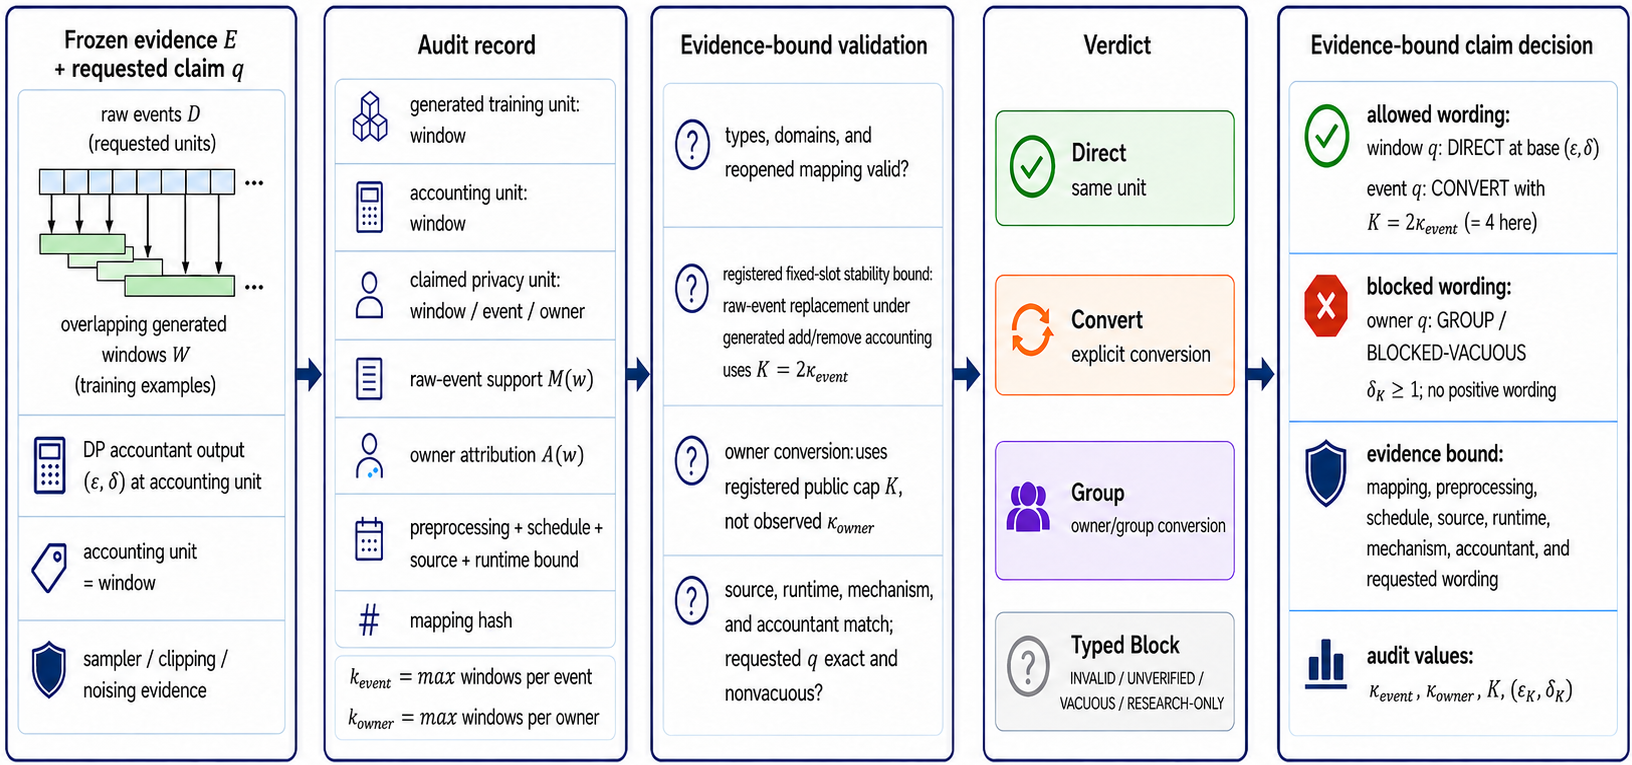
\includegraphics[width=\textwidth]{figures/ch02_source_evidence_validation.png}
    \caption{Evidence-bound validation and query separation for one frozen WISDM
    execution}
    \label{fig:ch2-evidence-validation-pipeline}
\end{figure}

\begin{lemma}[Query separation]
\label{lem:ch2-query-separation}
For fixed \(\EvidenceBundle\), suppose two requested claims satisfy
\(
\ClaimValidator(\EvidenceBundle,q_1)
\neq
\ClaimValidator(\EvidenceBundle,q_2)
\).
No query-oblivious interface \(A(\EvidenceBundle)\) can be exact for both
requests.
\end{lemma}

\begin{proof}[Proof]
The interface receives the same input for both requests and therefore has one
output distribution.  That distribution cannot be concentrated on two distinct
decision tuples.  Returning one common result is therefore incorrect for at least
one request; a common abstention is likewise inexact whenever either request is
licensed.  Hence exactness requires the requested claim to be supplied as an
input.
\end{proof}

Lemma~\ref{lem:ch2-query-separation} is an interface-separation result, not a new
privacy theorem.  It establishes why the query in
Equation~\eqref{eq:ch2-validator-decision} cannot be replaced by a display option
applied after an evidence-only verdict.  Figure~\ref{fig:ch2-evidence-validation-pipeline}
illustrates the consequence: one frozen execution can license two different
positive pairs and block a third sentence.  The next subsection specifies how a
registered distance \(K\) determines the converted pair and when the vacuity gate
forces \textsf{Blocked}.

\subsection{Privacy-Unit Conversion and Claim Blocking}
\label{subsec:privacy-unit-conversion}

Once the requested path has been identified, a conversion is licensed only by a
registered distance bound connecting the two adjacency relations.  Suppose the
bound execution is established as \((\varepsilon,\delta)\)-DP at generated-record
distance one and Equation~\eqref{eq:ch2-stability-bound} holds for an integer
\(K\geq1\).  Standard group privacy then gives

\begin{equation}
    \ConvertedEpsilon = K\varepsilon,
    \qquad
    \ConvertedDelta
    = \delta \sum_{i=0}^{K-1} e^{i\varepsilon}.
    \label{eq:ch2-group-conversion}
\end{equation}

Equation~\eqref{eq:ch2-group-conversion} is a registered consequence of the base
guarantee, not a new accountant or privacy theorem
\cite{dwork2014algorithmic}.  The validator neither estimates \(K\) from the
requested wording nor substitutes an observed incidence for a worst-case bound.
It first requires a registered transformation argument, then evaluates the
geometric sum with stable log-domain arithmetic.  For \(\varepsilon>0\), the
implementation uses

\begin{equation}
    \log \ConvertedDelta
    = \log\delta
    + \log\!\bigl(\operatorname{expm1}(K\varepsilon)\bigr)
    - \log\!\bigl(\operatorname{expm1}(\varepsilon)\bigr),
    \label{eq:ch2-stable-delta}
\end{equation}

with the exact \(\varepsilon=0\) limit \(\ConvertedDelta=K\delta\).  This avoids
overflow without changing the privacy consequence.  A public pair is emitted only
when both values are finite, \(\ConvertedEpsilon\geq0\), and
\(0<\ConvertedDelta<1\).  A non-finite result,
\(\ConvertedDelta\geq1\), or an unregistered derivation blocks positive wording.
The resulting values may remain visible as diagnostics, but their presence does
not convert a vacuous result into an allowed privacy claim; clamping delta to one
for serialization is not a privacy result.

\begin{proposition}[Contract-relative consequence]
\label{prop:ch2-contract-relative-consequence}
Assume that (i) \(\EvidenceBundle\) describes \(\DataTransform\) and the executed
mechanism \(\DPMechanism\); (ii) a registered checker establishes
\[
    \GeneratedAdjacencyMetric\!\left(
        \DataTransform(\RawDataset),
        \DataTransform(\RawDataset')
    \right) \leq K
\]
for every pair satisfying
\(\RawAdjacencyMetric(\RawDataset,\RawDataset')\leq1\); and (iii) a registered
accountant establishes \((\varepsilon,\delta)\)-DP for the bound execution at
generated-record distance one.  Then \(\DPMechanism\circ\DataTransform\) satisfies
Equation~\eqref{eq:ch2-group-conversion} for the requested raw adjacency.  If
\(K=1\) and the units and metrics coincide, the base pair takes the
\textsf{Direct} path.
\end{proposition}

\begin{proof}[Proof]
For a raw-adjacent pair, premise (ii) supplies a generated-metric path of length at
most \(K\) between the two transformed datasets.  Applying the distance-one DP
inequality successively along that path multiplies the likelihood factor by
\(e^{\varepsilon}\) at each step.  The additive terms accumulate with multipliers
\(1,e^{\varepsilon},\ldots,e^{(K-1)\varepsilon}\), which yields
Equation~\eqref{eq:ch2-group-conversion}.  When \(K=1\), the expression reduces to
the base pair.  The conclusion is conditional on the three registered premises;
the validator checks their disclosed evidence rather than proving execution
fidelity.
\end{proof}

The metric pair is essential when selecting \(K\).  A raw replacement can replace
several generated windows, but a replacement is one edit under a generated
replace-one metric and two edits under a generated add/remove metric.  This
distinction produces the factor-of-two case summarized in
Table~\ref{tab:ch2-adjacency-distance}.

\begin{corollary}[Factor-two mapping]
\label{cor:ch2-factor-two-mapping}
Assume public fixed-slot identities and a registered complete-support bound under
which one raw-event replacement changes at most \(\EventIncidence\) generated
records.  A generated add/remove accountant licenses
\(K=2\EventIncidence\), whereas a generated replace-one accountant licenses
\(K=\EventIncidence\).
\end{corollary}

\begin{proof}[Proof]
Each affected generated record is replaced.  Under add/remove distance, one such
replacement consists of one removal and one addition, so at most
\(2\EventIncidence\) edits are required.  Under replace-one distance, each
replacement costs one edit, giving \(\EventIncidence\).  The conclusion relies on
the registered complete-support premise; observed overlap alone is insufficient.
\end{proof}

These consequences produce four distinct decision cases.  A native-unit request
with coincident adjacency uses \(K=1\) and retains the base pair as
\textsf{Direct}.  A raw-event request takes \textsf{Convert} only when the event
stability argument and its metric-specific \(K\) are registered.  An owner request
takes \textsf{Group} when a public contribution bound supplies the generated
distance.  If no such bound is registered, the path is \textsf{Underspecified}; if
the bound exists but Equation~\eqref{eq:ch2-group-conversion} is non-finite or
vacuous, the path remains typed but the release is \textsf{Blocked}.

The WISDM evidence in Figure~\ref{fig:ch2-evidence-validation-pipeline}
illustrates why a public cap and an observed maximum are not interchangeable.  Its
fixed-slot event replacement has \(\EventIncidence=2\) and generated add/remove
accounting, so Corollary~\ref{cor:ch2-factor-two-mapping} gives \(K=4\).  For the
owner path, a public prefix policy caps contributions at 600 windows before
training.  The observed maximum of 565 verifies compliance with that policy but
does not replace it as a neighboring-dataset bound; the conversion therefore uses
\(K=600\).  Because the resulting \(\ConvertedDelta\) is at least one, the owner
path is reported as \textsf{Group}/\textsf{Blocked} and no positive owner-level
sentence is released.

The conversion rule thus determines what follows if the evidence premises hold;
it does not establish that the disclosed mapping, runtime, mechanism, and
accountant all belong to the same execution.  The next subsection specifies those
binding obligations and the assurance boundary of a bundle-only decision.

\subsection{Decision Procedure and Artifact Invalidation}
\label{subsec:evidence-binding-boundary}

The conversion consequence in Section~\ref{subsec:privacy-unit-conversion} is
meaningful only when the transformation, runtime, mechanism, and accountant
records refer to the same reported execution.  The validator therefore binds more
than a model artifact and a final privacy pair.  Its internal record includes the
selected mapping and identities; event support and owner attribution;
preprocessing, population, contribution, selection, and schedule policies;
mechanism, runtime, source, and accountant versions; base privacy parameters; and
the requested-unit contract.  The public view may redact private provenance, but
it retains the decision, artifact bindings, numerical result or diagnostic,
assumptions, forbidden wording, localized issues, and conditions that trigger
revalidation.

The finite-registry validator applies the following eight phases in order.  This
procedure is a typed evidence-to-wording decision, not a training algorithm.

\begin{enumerate}[label=(\arabic*),leftmargin=*,itemsep=3pt,topsep=4pt]
    \item \textbf{Types and domains.} Exact typed parsing rejects Boolean values
    supplied as integers, non-finite numerical values, invalid probabilities, and
    fields outside the registered domain before any privacy consequence is
    evaluated.

    \item \textbf{Reopened mapping.} The validator reopens the mapping rather than
    trusting a copied report string.  It recomputes file and semantic bindings,
    selected identities, intervals, event supports, owner attributions,
    \(\EventIncidence\), and \(\OwnerIncidence\).

    \item \textbf{Registered stability.} The selected checker must cover record
    identity and influence together with preprocessing, population, contribution,
    schedule, and selection dependencies.  A checker that covers only observed
    overlap does not establish Equation~\eqref{eq:ch2-stability-bound}.

    \item \textbf{Runtime agreement.} Observed fields must match the registered
    sampler, sampling rate, optimization steps, noise and clipping rules,
    accounting unit, mapping and pipeline identities, and secure-randomness mode.
    Missing runtime observation blocks concrete-run wording.

    \item \textbf{Registry binding.} A versioned registry binds supported source
    and adapter identities to the mechanism semantics and accountant.  The
    validator recomputes the base pair and default-denies unknown adapters,
    attachments, or accounting rules.

    \item \textbf{Path resolution.} The requested unit and adjacency select the
    direct, converted, grouped, or underspecified path and its registered
    stability method.  The validator never infers a path from the wording alone.

    \item \textbf{Numerical consequence.} The base pair is retained only on the
    exact native path.  Otherwise Equations~\eqref{eq:ch2-group-conversion}
    and~\eqref{eq:ch2-stable-delta} are evaluated under the registered \(K\).

    \item \textbf{Typed release.} Exact wording, issue precedence, the non-finite
    and vacuity gates, and the authority label determine the public report.  The
    operational metadata may be redacted without changing that decision.
\end{enumerate}

Four complementary digests support these checks.  A full-file digest detects byte
substitution.  A canonical selected digest binds the normalized semantic records
that participate in the run, so permutation or irrelevant decoy rows cannot
silently redefine the selected mapping.  A pipeline digest binds transformation
and policy parameters, and a runtime digest binds the observed mechanism fields.
These digests expose changed, stale, or mutually inconsistent artifacts.  They do
not establish that the producer executed the referenced bytes: equal mapping
digests do not prove sampler use, and equal report text cannot replace reopening
the underlying files.  Changing a bound mapping, selected identity, preprocessing
or population rule, contribution policy, schedule, mechanism or accountant
version, runtime parameter, claim unit, adjacency, or conversion method therefore
invalidates the old report and triggers validation again.  A redacted public view
is a view of the same decision, not a separately certified claim.

When several conditions apply, the implemented release precedence is

\begin{equation}
\begin{split}
    \textsf{Blocked-Invalid} &\;>\; \textsf{Blocked-Unverified}
    \;>\; \textsf{Blocked-Vacuous} \\
    &\;>\; \textsf{Research-Only} \;>\; \textsf{Allowed}.
\end{split}
\label{eq:ch2-release-precedence}
\end{equation}

The ordering prevents a valid scalar calculation from masking a malformed input
or missing runtime trace.  Likewise, an external attachment cannot repair an
unrelated mechanism contradiction, and a blocked internal diagnostic cannot be
converted into an allowed public sentence by redaction.

\subsection{Evidence Authority, Complexity, and Non-Attestation Boundary}
\label{subsec:ch2-evidence-authority}

The validation cost is dominated by reopening and checking these structures.  For
\(B\) mapping bytes, \(R\) rows, \(S\) selected rows, \(A\) attribution entries,
and \(P\leq2A\) interval endpoints, the registered checks require
\(O(B+R+A+S\log S+P\log P)\) time and \(O(R+A)\) memory, in addition to the work
of the registered accountant.  This bound describes the complete validator; a
specialized aggregate rescan that checks only mapping statistics is not an
equivalent certificate.

The remaining assurance boundary is informational.  A bundle-only validator can
test consistency among the objects it receives, but unauthenticated self-reporting
cannot distinguish faithful execution from a producer that presents the same
bundle after executing different code or hiding a dependency.

\begin{proposition}[Bundle-only non-attestation]
\label{prop:ch2-bundle-only-non-attestation}
Let a validator observe only an unauthenticated tuple
\((\EvidenceBundle,\ClaimQuery,\ValidationRegistry)\).  Suppose a faithful world
and a world that reports the same tuple while executing different code or hiding
a dependency are observationally identical to the validator.  Every deterministic
or randomized validator has the same output distribution in both worlds and
therefore cannot establish execution fidelity from that tuple alone.
\end{proposition}

\begin{proof}[Proof]
The validator receives identical inputs in the two worlds.  A deterministic
validator must consequently return the same output, and a randomized validator
must induce the same conditional output distribution.  No decision rule over the
observed tuple can separate the worlds without an additional authenticated
observation.
\end{proof}

The threat model is consequently an honest-but-fallible producer: stale exports,
omitted dependencies, inconsistent configuration, mismatched artifacts, and
unjustified privacy-unit restatement are in scope.  A malicious producer that can
fabricate a mutually consistent bundle while running another procedure is outside
the positive assurance claim.  Addressing that adversary requires authenticated
runtime observation, execution attestation, or a cryptographic proof system
\cite{narayan2015verifiable,shamsabadi2024confidential}.  The experiments in the
next section test whether the registered observable obligations separate designed
allowed and non-allow cases; they do not measure faithful execution.  In this
chapter, \textsf{EVIDENCE\_VALIDATED} means that registered observable obligations
pass; it does not mean execution fidelity.

\section{Experimental Evaluation}
\subsection{Controlled Validation and Ablation}
\label{subsec:controlled-validation-ablation}

The first experimental question is which claim distinctions disappear when the
validator observes only a weak projection of the evidence or when a registered
obligation is removed.  The controlled suite contains 100 allowed cases spanning
five registered path strata---direct window, direct event, direct owner,
converted event, and grouped owner---at five boundary or scale levels and in four
mapping contexts.  The contexts include a canonical mapping, irregular supports,
non-selected decoy rows, and permuted file order.  Each allowed parent is paired
with one non-allow case.  The 100 paired cases are produced by 25 one-premise
mutation operators, each applied to four distinct parents, so that every allowed
parent is consumed once.

An authored manifest, rather than the output of the full validator, declares the
expected path, release and assurance state, localized issue, and numerical rule.
Every method receives the same report, audit row, and mapping.  The
\emph{unsafe-positive fraction} is the fraction of the 100 non-allow cases that
nevertheless receive an allowed decision.  The \emph{valid-exact fraction} is the
fraction of the 100 allowed cases for which both the decision path and privacy
pair are exact.  The \emph{exact-tuple fraction} is evaluated over all 200 cases
and additionally requires the correct assurance state, block subtype, and
presence or absence of numerical output.  These fractions are deterministic
coverage outcomes for the authored suite.  They are neither estimates of a
deployment population nor empirical error rates.

Table~\ref{tab:ch2-controlled-ablation} compares the complete registered contract
(\textsf{FULL}) with two kinds of deliberately weakened checks.  B0--B4 are
information projections that retain only field presence, JSON Schema validity,
multiplicity, mapping-hash binding, or base-accountant recomputation.  A1 leaves
the static contract intact but assumes that runtime evidence matches it, whereas
A2 removes only the vacuity gate.  The rows are therefore diagnostic projections
and obligation ablations, not predecessor systems or competing validators.

\begin{table}[tbp]
    \centering
    \caption{Controlled-suite and ablation results}
    \label{tab:ch2-controlled-ablation}
    \footnotesize
    \setlength{\tabcolsep}{2.3pt}
    \renewcommand{\arraystretch}{1.13}
    \begin{tabular}{@{}
        >{\raggedright\arraybackslash}p{0.19\textwidth}
        >{\centering\arraybackslash}p{0.105\textwidth}
        >{\centering\arraybackslash}p{0.105\textwidth}
        >{\centering\arraybackslash}p{0.105\textwidth}
        >{\raggedright\arraybackslash}p{0.31\textwidth}@{}}
        \toprule
        \textbf{Probe / full contract} &
        \textbf{Unsafe-positive frac.} &
        \textbf{Valid-exact frac.} &
        \textbf{Exact-tuple frac.} &
        \textbf{Principal evidence not checked} \\
        \midrule
        B0 Field presence &
        1.00 & 0.60 & 0.00 &
        types, semantics, files, execution, accounting \\

        B1 JSON Schema &
        0.96 & 0.60 & 0.00 &
        cross-field and execution semantics \\

        B2 Multiplicity only &
        1.00 & 0.80 & 0.00 &
        stability/adjacency, staleness, mechanism \\

        B3 Hash only &
        0.96 & 0.60 & 0.00 &
        consistently wrong semantics or mechanism \\

        B4 Accountant only &
        0.88 & 0.60 & 0.00 &
        mapping, claimed unit, dependencies, runtime \\

        A1 Runtime assumed matched &
        0.12 & 1.00 & 0.94 &
        independent runtime/artifact equality \\

        A2 \textsf{FULL} minus vacuity &
        0.04 & 1.00 & 0.98 &
        reportability of converted numerics \\

        \textsf{FULL} &
        \textbf{0.00} & \textbf{1.00} & \textbf{1.00} &
        registered-contract assurance boundary \\
        \bottomrule
    \end{tabular}
\end{table}

The complete contract produces no unsafe positive among the 100 paired
non-allow cases, exactly matches all 100 allowed cases, and returns the expected
full tuple in all 200 cases.  An independent standard-library implementation of
the grid and mutation oracle passes 20,909 of 20,909 checks, and the expanded
contract suite passes 83 of 83 checks.  These checks establish conformance to the
finite authored contract, not correctness for an unregistered mechanism or
unobserved execution.

The weaker rows expose distinct losses of information.  B0, B1, B3, and B4 reuse
the base privacy pair in 40 allowed conversion or grouping cases, while B2 does so
in four.  A1 retains every allowed case but leaves 12 unsafe positives: four each
for missing-trace, runtime-noise, and runtime-artifact mutations.  A2 leaves four
vacuous owner-level positives.  Five fixed necessity witnesses isolate the
corresponding obligations: reopened mapping bytes, registered stability status,
runtime noise and trace equality, the vacuity gate, and exact event rather than
window wording.  Removing each obligation erases the decision boundary between
its paired valid and blocked witness.  Independent recomputation passes all 10
witness decisions as well as their associated tamper tests.

\begin{table}[tbp]
    \centering
    \caption{Fixed information-necessity witnesses}
    \label{tab:ch2-necessity-witnesses}
    \footnotesize
    \setlength{\tabcolsep}{2.8pt}
    \renewcommand{\arraystretch}{1.13}
    \begin{tabular}{@{}
        >{\centering\arraybackslash}p{0.07\textwidth}
        >{\raggedright\arraybackslash}p{0.26\textwidth}
        >{\raggedright\arraybackslash}p{0.27\textwidth}
        >{\raggedright\arraybackslash}p{0.30\textwidth}@{}}
        \toprule
        \textbf{ID} & \textbf{Fixed comparison} &
        \textbf{Deleted or hidden edge} & \textbf{Required distinction} \\
        \midrule
        W1 & Valid parent P01 vs. blocked F02 &
        Actual mapping bytes; report, audit row, and query held equal &
        \textsf{Allowed} vs. \textsf{Blocked-Invalid} \\

        W2 & Converted parent P02 vs. F16 &
        Registered stability status; remaining public fields held equal &
        \textsf{Convert/Allowed} vs. \textsf{Blocked-Unverified} \\

        W3 & Direct parent P01 vs. F05 &
        Runtime noise and trace equality &
        \textsf{Direct/Allowed} vs. \textsf{Blocked-Invalid} \\

        W4 & F01 under A2 vs. \textsf{FULL} &
        Vacuity and reportability gate &
        Unsafe owner positive vs. typed vacuous block \\

        W5 & One WISDM event certificate &
        Exact licensed event sentence replaced by a valid window sentence &
        Independent wording verifier rejects the substitution \\
        \bottomrule
    \end{tabular}
\end{table}

Table~\ref{tab:ch2-necessity-witnesses} is intentionally narrower than a universal
minimality claim.  The witnesses show that deleting one named edge loses a
required distinction on authenticated fixed inputs; they do not prove that every
audit engine must use the same files or that such failures occur at a measured
rate in published systems.

A second authority source avoids relying only on newly authored mutations.  A
protocol fixed before the conformance construction identified ten preserved
development incidents whose root causes affected claim-bearing output and had
pre-protocol discovery records.  A production-import-free verifier reopens the
historical source or archive member, discovery anchor, consequence, and 16 repaired
controls, passing 176 of 176 checks.  Three tamper tests retain the authentic
lineage and reject an omitted incident or forged archive identity.  This is actual
development lineage from the evaluated system, but it is not an independently
sampled publication corpus and therefore does not estimate real-world prevalence.

For scope comparison, the official TensorFlow Privacy 0.9.0 privacy-statement
function \cite{google2024tfprivacy} is evaluated on the original 23-case subset
that can be expressed through its scalar interface.  Given caller-supplied
scalars and a group bound, it returns finite conditional statements for all seven
valid cases and for 15 of 16 non-allow bundles; it rejects a Boolean value supplied
for the number of steps.  All 79 reproduction checks re-execute and hash the
official module and setup.  In the fixed-base vacuity case, the function solves a
smaller example-level delta and freshly targets a user-level delta.  This is a
useful alternative accounting contract, but it is not
Equation~\eqref{eq:ch2-group-conversion} applied to the supplied privacy pair.
Accordingly, the comparison is not a quality ranking: the scalar function derives
a conditional statement from values supplied by its caller, whereas
\textsf{FULL} reopens the pipeline evidence and decides whether the exact
submitted tuple supports the requested sentence.  The next subsection tests that
evidence-bound distinction on activity data and mapping-only rescans.

\subsection{Complete Activity-Data Executions}
\label{subsec:activity-mapping-validation}

The second experimental question asks whether one frozen evidence bundle produces
distinct query-dependent decisions and whether that pattern recurs across fresh,
separately bound executions.  The complete activity-data path uses the public
WISDM accelerometer data \cite{kwapisz2011activity}.  A public parser reduces
1,098,210 physical lines to 1,086,465 canonical valid events.  From these events,
the registered transformation constructs 7,304 training windows, each with length
200 and stride 100.  Owner identities partition the mapping, feature and label transforms
are record-local, and a public prefix policy caps training-window contributions at
600 per owner before training.  The bound run uses Poisson window sampling at
\(1/50\), 100 optimization steps, and noise multiplier 2.  Registered RDP
recomputation yields the base pair
\((0.536827391167,10^{-6})\).

Every request in Table~\ref{tab:ch2-wisdm-query-decisions} reopens the same
7,304-row mapping and binds the same pipeline and runtime evidence.  The window
query is native to the accountant and therefore uses \(K=1\).  Under fixed-slot
raw-event replacement, the reopened mapping gives
\(\EventIncidence=2\); because the base metric is generated add/remove,
Corollary~\ref{cor:ch2-factor-two-mapping} gives \(K=4\).  The owner request
observes a maximum contribution of 565 only as a compliance check.  Its registered
conversion uses the public cap \(K=600\), not that observed maximum.

\begin{table}[tbp]
    \centering
    \caption{Query-dependent decisions for one frozen WISDM execution}
    \label{tab:ch2-wisdm-query-decisions}
    \small
    \setlength{\tabcolsep}{3pt}
    \renewcommand{\arraystretch}{1.15}
    \begin{tabular}{@{}
        >{\raggedright\arraybackslash}p{0.17\textwidth}
        >{\centering\arraybackslash}p{0.17\textwidth}
        >{\raggedright\arraybackslash}p{0.23\textwidth}
        >{\raggedright\arraybackslash}p{0.29\textwidth}@{}}
        \toprule
        \textbf{Requested claim} &
        \textbf{Observed / registered (K)} &
        \textbf{Path / release} &
        \textbf{Pair or action} \\
        \midrule
        Window &
        -- / 1 &
        \textsf{Direct} / \textsf{Allowed} &
        \((0.53683,10^{-6})\) \\

        Raw event &
        2 / 4 &
        \textsf{Convert} / \textsf{Allowed} &
        \((2.14731,1.0642\times10^{-5})\) \\

        Owner &
        565 / 600 &
        \textsf{Group} / \textsf{Blocked} &
        vacuous: \(\delta_K\geq1\) \\
        \bottomrule
    \end{tabular}
\end{table}

Thus the same execution licenses the base window sentence, licenses a weaker
event-level sentence after registered conversion, and withholds positive
owner-level wording.  The owner path remains \textsf{Group}; its release is
separately \textsf{Blocked} because Equation~\eqref{eq:ch2-group-conversion}
produces \(\varepsilon_K=322.096\).  Its converted delta satisfies
\(\log_{10}\delta_K=134.033097\), and hence \(\delta_K\geq1\).  The existence of those
diagnostic numbers does not make them reportable privacy parameters.

Five post-freeze WISDM runs have distinct model digests and preserve all three
decision paths and privacy values.  Across those runs, accuracy is
\(0.6556\pm0.0080\) and macro-F1 is \(0.3922\pm0.0033\).  A separately bound
The complete pipeline---raw parsing, mapping, training, report generation, and
evidence production---takes \(16.743\pm1.191\) seconds over the five runs in the
reported environment.  Independent verification with raw reconstruction takes
\(6.480\pm0.428\) seconds.  Five additional portable invocations take
\(1.577\pm0.125\) seconds and pass 35 of 35 checks each while omitting the three
raw-input reconstruction checks.  A complete run directory averages 0.996 MB;
the separately acquired 50.326 MB raw file is required only for full-source
reconstruction.  These end-to-end timings include process startup and are not
isolated validator overhead.

A separately bound route uses the UCI Human Activity Recognition Using Smartphones data
\cite{anguita2013har,reyesortiz2013uci}, with 7,352 training windows, 2,947 test
windows, and 561 features.  Each of five post-freeze runs passes 49 of 49
raw-source checks and 38 of 38 portable checks with a distinct digest.  Because
event support and an owner contract are absent, each run licenses only
\textsf{Direct} window add/remove wording at approximately
\((0.536827,10^{-6})\); event and owner requests are blocked rather than inferred.
Its mean accuracy is \(0.8049\pm0.0315\), and mean macro-F1 is
\(0.7795\pm0.0504\).  Both datasets' accuracy and F1 values are integration
diagnostics, not competitive or state-of-the-art utility claims.

\begin{table}[H]
    \centering
    \caption{Invariant UCI HAR authorization boundary across five executions}
    \label{tab:ch2-uci-authorization}
    \small
    \setlength{\tabcolsep}{5pt}
    \renewcommand{\arraystretch}{1.15}
    \begin{tabular}{@{}
        >{\raggedright\arraybackslash}p{0.20\textwidth}
        >{\centering\arraybackslash}p{0.22\textwidth}
        >{\centering\arraybackslash}p{0.22\textwidth}
        >{\centering\arraybackslash}p{0.12\textwidth}@{}}
        \toprule
        \textbf{Requested unit} & \textbf{Release status} &
        \textbf{Path} & \textbf{\(K\)} \\
        \midrule
        Published window & \textsf{Allowed} & \textsf{Direct} & 1 \\
        Raw event & \textsf{Blocked-Unverified} & \textsf{Underspecified} & -- \\
        Owner & \textsf{Blocked-Unverified} & \textsf{Underspecified} & -- \\
        \bottomrule
    \end{tabular}
\end{table}

Table~\ref{tab:ch2-uci-authorization} is invariant across all five protocol-fixed
runs.  This negative result is informative: an existing published-window dataset
does not automatically expose the raw-session support or public owner cap needed
for a stronger unit claim, even when the DP-SGD mechanism and accountant are
otherwise reproduced.

\subsection{Sepsis and Backblaze Mapping Diagnostics}
\label{subsec:ch2-mapping-diagnostics}

The third experimental question isolates the transformation side of the contract
at substantially larger scales.  For
the PhysioNet/Computing in Cardiology 2019 Sepsis data
\cite{goldberger2000physiobank,reyna2019sepsis,reyna2020sepsis}, the verifier
opens and hashes 5,000 patient files and reconstructs 16 mappings under dense,
non-overlap, and public-cap policies.  For the Backblaze first-quarter 2025 drive
statistics \cite{backblaze2025stats}, a verifier without production imports
rescans 1.02 GB comprising 90 daily files, 27,799,986 drive-day rows, and 318,426
drives.  It distinguishes windows over ordered available snapshots, which may
compress calendar gaps, from calendar-contiguous windows.

The Sepsis source contains 192,206 hourly patient rows.  Six-, twelve-, and
twenty-four-hour window policies cover dense, half-stride, and non-overlap
schedules, while public owner-local prefix caps of 1, 4, 8, and 16 make the
contribution rule observable before selection.  Label-balanced caps act as
negative controls: they can reproduce the same displayed counts as a public
prefix cap while using private labels to change selected identities.  Candidate
event distance is therefore reported only for fixed positional or public-prefix
policies whose support premise is registered.

The Backblaze rescan covers 27,799,986 unique drive-day events with no duplicate
serial-number and date pair and evaluates 22 mapping policies.  Ordered-snapshot and
calendar-contiguous windows can display equal incidence while selecting different
records; public owner-prefix caps are evaluated separately.  This distinction is
why a compact table can summarize representative rows but cannot replace the full
policy identity bound into the mapping evidence.

\begin{table}[tbp]
    \centering
    \caption{Mapping-only diagnostics for Sepsis and Backblaze data}
    \label{tab:ch2-mapping-only-diagnostics}
    \footnotesize
    \setlength{\tabcolsep}{2.8pt}
    \renewcommand{\arraystretch}{1.12}
    \begin{tabular}{@{}
        >{\raggedright\arraybackslash}p{0.10\textwidth}
        >{\raggedright\arraybackslash}p{0.29\textwidth}
        >{\raggedleft\arraybackslash}p{0.14\textwidth}
        >{\centering\arraybackslash}p{0.09\textwidth}
        >{\centering\arraybackslash}p{0.11\textwidth}
        >{\centering\arraybackslash}p{0.09\textwidth}@{}}
        \toprule
        \textbf{Dataset} &
        \textbf{Mapping policy} &
        \textbf{Generated records} &
        \textbf{Obs. \(\EventIncidence\)} &
        \textbf{Candidate event \(K\)} &
        \textbf{Obs. \(\OwnerIncidence\)} \\
        \midrule
        Sepsis & 6h dense & 167,206 & 6 & 12 & 331 \\
        Sepsis & 6h non-overlap & 29,958 & 1 & 2 & 56 \\
        Sepsis & public owner cap 1 & 5,000 & 1 & 2 & 1 \\
        \midrule
        Backblaze & 7d dense, ordered snapshots & 25,904,370 & 7 & 14 & 84 \\
        Backblaze & 7d dense, calendar-contiguous & 25,867,949 & 7 & 14 & 84 \\
        Backblaze & 7d non-overlap, ordered & 3,709,484 & 1 & 2 & 12 \\
        Backblaze & 7d non-overlap, calendar & 3,707,669 & 1 & 2 & 12 \\
        Backblaze & 60d non-overlap, ordered & 304,906 & 1 & 2 & 1 \\
        Backblaze & 60d non-overlap, calendar & 302,760 & 1 & 2 & 1 \\
        \bottomrule
    \end{tabular}
\end{table}

The Sepsis and Backblaze verifiers pass 128 of 128 and 86 of 86 checks,
respectively.  Table~\ref{tab:ch2-mapping-only-diagnostics} nevertheless exposes
three distinct premise risks.  First, non-overlap can reduce
\(\EventIncidence\) to one while fixed-slot replacement under generated
add/remove accounting still gives candidate \(K=2\).  Second, ordered and
calendar-contiguous Backblaze semantics differ by 36,421 dense seven-day windows
despite equal incidence.  Third, a Sepsis label-balanced selection can reproduce
public-cap counts while privately changing selected identities.  The rescans
reconstruct rows and policies, but neither bundle binds a mechanism, runtime, or
accountant.  Consequently, every row is only a mapping diagnostic: no row is an
\((\varepsilon,\delta)\) certificate or a \textsf{Direct} verdict, and no positive
privacy wording is emitted.

\subsection{Independent Verification, External Intake, and Reproducibility}
\label{subsec:ch2-independent-verification}

The final experimental question asks whether each result can be reconstructed
without merely importing the production validator.  Separate implementations
reopen the relevant inputs, recompute hashes, rows, decisions, and numerical
tolerances, and confirm that a blocked public output contains no positive
sentence.  Table~\ref{tab:ch2-verification-surfaces} reports the principal
surfaces.  The denominators enumerate deterministic assertions in fixed artifacts;
they are not confidence intervals or independent human replications.

\begin{table}[tbp]
    \centering
    \caption{Independent verification surfaces and stated authority}
    \label{tab:ch2-verification-surfaces}
    \footnotesize
    \setlength{\tabcolsep}{3pt}
    \renewcommand{\arraystretch}{1.13}
    \begin{tabular}{@{}
        >{\raggedright\arraybackslash}p{0.34\textwidth}
        >{\centering\arraybackslash}p{0.18\textwidth}
        >{\raggedright\arraybackslash}p{0.37\textwidth}@{}}
        \toprule
        \textbf{Surface} & \textbf{Passing checks} &
        \textbf{Authority} \\
        \midrule
        Expanded contract regression & 83/83 &
        Fixed schema, registry, and release semantics \\
        Designed 200-case conformance surface & 20,909/20,909 &
        Five strata, 25 operators, fixed oracle and lineage \\
        Necessity witnesses & 10/10 &
        Five fixed edge-deletion distinctions \\
        Retrospective development lineage & 176/176 &
        Ten preserved incidents and 16 repaired controls \\
        TensorFlow Privacy scope comparison & 79/79 &
        Re-execution and hashing of the official scalar interface \\
        WISDM reference and each confirmatory run & 38/38 &
        Full raw reconstruction and three query decisions \\
        UCI HAR full / portable, each run & 49/49 / 38/38 &
        Published-input reconstruction / distributable evidence \\
        Sepsis / Backblaze mapping rescans & 128/128 / 86/86 &
        Mapping and policy diagnostics only \\
        \bottomrule
    \end{tabular}
\end{table}

An externally authored ExtraSensory source-path intake provides a separate
authority test \cite{loya2022extrasensory,vaizman2017context}.  Six terminal
records are retained rather than reporting only the successful attempt: repository
import, path, disk, loader, and plotting failures precede one complete five-epoch
execution.  The final run produces all 17 expected outputs, and separate verifiers
reconstruct its mapping and execution records.  Nevertheless, the external source
sets \texttt{secure\_rng=False} and prints a configured target epsilon rather than
an accountant-derived achieved epsilon.  The terminal result is therefore
execution-complete but claim-unverified; positive DP wording remains empty.  This
case demonstrates why successful training and artifact presence are not sufficient
authority for a privacy sentence.

The reproducibility package pins the core Python dependencies, schemas, registry,
claim-bearing reports, frozen outputs, and verification entry points.  Every
reported table row has a machine-readable source, while larger public datasets are
identified by acquisition boundary and digest rather than redistributed.  Exact
frozen-number verification does not require retraining; fresh WISDM runs use new
private randomness, so the verifier requires internal consistency and invariant
decision semantics rather than identical model or batch-trace hashes.  No
nondeterministic outcome is silently dropped, and missing raw inputs, unregistered
adapters, research randomness, private-dependent selection, and vacuous conversion
remain typed limitations rather than being converted into positive results.

\section{Summary}
\label{sec:ch2-summary-transition}

This chapter treated a privacy statement as a query over frozen execution
evidence rather than as a synonym for an accountant output.  The validator first
checks whether the requested unit and adjacency are connected to the generated
records, mechanism, runtime, and accountant through a registered evidence chain.
It then reports a typed path and independently decides whether positive wording is
allowed.  As a result, one completed execution can support a native-unit claim,
support a weaker converted claim, and block a stronger claim without collapsing
those outcomes into one privacy label.

The resulting assurance is deliberately bounded.  It is relative to the supplied
evidence and a finite validation registry; it is not execution attestation, an
arbitrary-code proof, or a new accountant.  Reopened artifacts, semantic digests,
runtime equality, registered stability, recomputation, and fail-closed release
reduce accidental claim--evidence mismatches under the honest-but-fallible threat
model.  They cannot distinguish faithful execution from a producer that presents
a consistently fabricated bundle.  Missing, unregistered, non-finite, or vacuous
premises therefore suppress positive wording rather than justify extrapolation.

The practical conclusion is a reuse boundary.  A completed model may be reused
with the exact native or converted wording licensed by its evidence, but a blocked
patient- or owner-level request cannot inherit the window-level pair.  Satisfying
that stronger request requires additional registered premises or a new mechanism
and execution native to the requested unit.  Chapter~\ref{ch:pp-mark} turns from
privacy wording to generative-image provenance.  The assurance object changes,
but the same dissertation-level question remains: whether a public decision is
supported by the target, mechanism, interface, and evidence that the decision
claims to represent.
